\chapter{The two smoothings of \texorpdfstring{$C(\dP6)$}{C(dP6)}}
%\chapter[The two smoothings of $\C(\dP6)$][The two smoothings of C(dP6)]{The two smoothings of $\boldsymbol{C(\dP6)}$}

In this chapter we study the toric singularity that is the cone over the del Pezzo surface of degree $6$. it has two topologically different smoothings, which we haven't seen studied in some detail before. 

\section{The del Pezzo surface \texorpdfstring{$\dP6$}{dP6}}
\label{sec:twosmoothings}

Denote by $\dP6$ the blow-up of $\P^2$ in three generic points.  These points can be chosen to be the coordinate points $(1:0:0),(0:1:0)$ and $(0:0:1)$. The torus action on $\P^2$ extends to an action on $\dP6$, so it is a toric variety.

\begin{figure}[b]
\centering 
\subbottom[The hexagon corresponding to $\dP6$.]{%
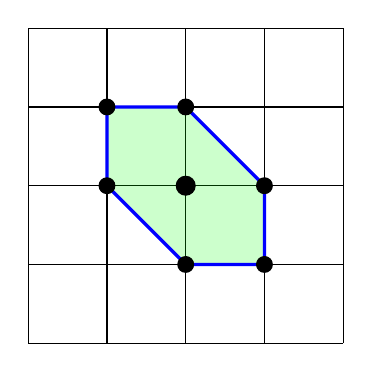
\begin{tikzpicture}
  \draw (0, 0) grid (4, 4);  
 
\draw [very thick, color=blue, fill=green, fill opacity=0.2]
(2,1) -- (3,1) -- (3,2) -- (2,3) -- (1,3) -- (1,2) -- cycle;

\draw [fill=black]  (2, 1) circle (0.1);
\draw [fill=black]  (3, 1) circle (0.1);
\draw [fill=black]  (3, 2) circle (0.1);
\draw [fill=black]  (2, 3) circle (0.1);
\draw [fill=black]  (1, 3) circle (0.1);
\draw [fill=black]  (1, 2) circle (0.1);
\draw [fill=black]  (2, 2) circle (0.12);
\end{tikzpicture}
%\caption{The hexagon.}
\label{fig:hexagon_dp6}
}
\subbottom[The fan over the polar polytope.]{%
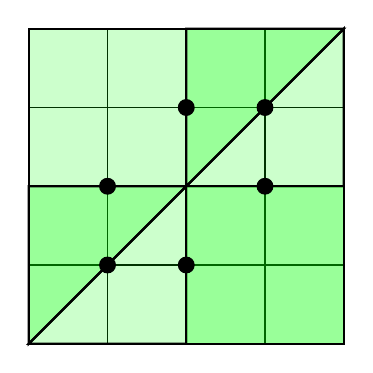
\begin{tikzpicture}
  \draw (0, 0) grid (4, 4);  
%\draw [very thick, fill=green, fill opacity=0.2]
%(1,1) -- (2,1) -- (3,2) -- (3,3) -- (2,3) -- (1,2) -- cycle;
\draw [thick,fill=green, fill opacity=0.2] (2,2) -- (4,2) -- (4,4) -- cycle;
\draw [thick,fill=green, fill opacity=0.4] (2,2) -- (4,4) -- (2,4) -- cycle;
\draw [thick,fill=green, fill opacity=0.2] (2,2) -- (2,4) -- (0,4) -- (0,2) -- cycle;
\draw [thick,fill=green, fill opacity=0.4] (2,2) -- (0,2) -- (0,0) -- cycle;
\draw [thick,fill=green, fill opacity=0.2] (2,2) -- (0,0) -- (2,0) -- cycle;
\draw [thick,fill=green, fill opacity=0.4] (2,2) -- (2,0) -- (4,0) -- (4,2) -- cycle;

\draw [fill=black]  (1, 1) circle (0.1);
\draw [fill=black]  (2, 1) circle (0.1);
\draw [fill=black]  (3, 2) circle (0.1);
\draw [fill=black]  (3, 3) circle (0.1);
\draw [fill=black]  (2, 3) circle (0.1);
\draw [fill=black]  (1, 2) circle (0.1);
%\draw [fill=black]  (2, 2) circle (0.1);
\end{tikzpicture}
%\caption{The fan of $dP_6$.}
\label{fig:fandp6}
}
\caption{Toric description of $dP_6$.}
\end{figure}

As a toric variety, it can be described as the toric variety corresponding to the polytope in \cref{fig:hexagon_dp6}. Its fan is depicted in \cref{fig:fandp6}. One can read off the Picard group of $\dP6$ from the fan, using the exact sequence
$$
0 \to \Z \xrightarrow{A} \Z^6 \to \Pic(\dP6) \to 0,
$$
where the matrix $A$ contain the primitive ray generators of the fan. This is Theorem 4.2.1 in \cite{cox_toric}. The cokernel is $\Pic(\dP6)=\Z^4$, which can also be seen directly from the description of $\dP6$ as a blowup.

There are several ways to describe the equations of $\dP6$. Since $\dP6$ is the blowup of $\P^2$ in three points, we can blow them up separately. Let $x_0,x_1,x_2$ be coordinates of $\P^2$. Then the blowup of $\P^2$ in the point $(1:0:0)$ can be realized as the closed subscheme of $\P^2 \times \P^1$ given by the equation $r_0x_1-r_1x_2=0$, where $r_0,r_1$ are coordinates on $\P^1$. We can repeat this procedure on the two other points $(0:1:0)$ and $(0:0:1)$ to obtain similar equations. Collecting these, we see that $\dP6$ is given by the matrix equation
\[
M\vec x = 
\begin{pmatrix}
0 & r_0 & -r_1 \\
s_1 & 0 & -s_0 \\
-t_0 & t_1 & 0
\end{pmatrix}
\begin{pmatrix}
x_0 \\ y_0 \\ z_0
\end{pmatrix}= 0.
\]
in $\P^2 \times \P^1 \times \P^1 \times \P^1$. Consider the projection forgetting the $\P^2$-factor:
$$
\pi:\P^2 \times \P^1 \times \P^1 \times \P^1 \to \P^1 \times \P^1 \times \P^1.
$$

 Note that the matrix cannot have rank $1$ or lower.  This means that the restriction of $\pi$ to $\dP6$ is an isomorphism onto the hypersurface given by $\det M=0$ in $\P^1 \times \P^1 \times \P^1$.

On the other hand, blowups can also be realized as closures of graphs of rational maps. Let $\varphi: \P^2 \rmap \P^2$ be the Cremona transformation given by $(x_0:x_1:x_2) \mapsto \left( \frac 1{x_0}: \frac 1{x_1}:\frac 1{x_2} \right)$. Then, in coordinates $(a_0:a_1:a_2) \times(b_0:b_1:b_2)$ on $\P^2 \times \P^2$, the equations $a_0b_0=a_1b_1=a_2b_2$ hold \label{eq:dp6_inp2p2}. These are the equations of the blowup along the indeterminacy locus of the rational map $\varphi$. The indeterminacy locus is exactly the three coordinate points. Hence $\dP6$ can also be realized as the intersection of two $(1,1)$-divisors in $\P^2 \times \P^2$. 

Hence, using the Segre embedding, $\dP6$ lives naturally in both ${\left( \P^1 \right)}^3 \hookrightarrow \P^7$ and $\P^2 \times \P^2 \hookrightarrow \P^8$. 

\begin{remark}
Intersecting $\P^2 \times \P^2$ with a single $(1,1)$-divisor gives us the projective space bundle corresponding to the tangent bundle of $\P^2$, which we denote by $\mathcal T(\P^2)$. This follows from the exact sequence
\[
0 \to \OO_{\P^2} \to {\OO_{\P^2}(1)}^3 \to \mathcal T_{\P^2} \to 0.
\]
Since $\P({\OO_{\P^2}(1)}^3)=\P^2$,  $\P(\mathcal T_{\P^2})$ can be realized as the subset of $\P^2 \times \P^2$ such that $a_0b_0+a_1b_1+a_2b_2=0$.
\todo{can the topology of this space be studied using e.g. chern classes?}
\end{remark}


\section{The cone over \texorpdfstring{$\dP6$}{dP6} and its two smoothings}

The singularity $Z=C(\dP6)$ is one of the most studied singularities with an obstructed deformation space, In the paper \cite{altmann_versaldeformation}, Altmann describe a method to study the versal deformations of isolated affine Gorenstein toric singularities using only the combinatorial data of the toric variety. He shows that different components of the base space correspond to different ways of writing the defining polytope as a Minkowski sum of other polytopes.

See the illustation in [[TO COME]].

\todo{illustration of $\dP6$ as a minkowski sum of different things}

Let $A=A(Z)$ denote the affine coordinate ring of $C(\dP6)$. It has a natural $\Z$-grading. From Altmann's article, or by using \MM, it is possible to compute that $\dim T^1(A)=3$, and that $\dim T^2(A)=2$. The versal base space decomposes into a union of a line and a plane.

For well-behaved singularities, often one can describe all of its deformations by writing up a ``format'' of the equations. For example, for codimension three Gorenstein projective schemes, there is a structure theorem for the whole resolution, involving pfaffians. For codimension $4$, there is no such result, though there have been some research in this direction \todo{cite Reid}.

It is worthwhile to note that both smoothings of $Z$ arise by ``sweeping out the cone'': if $X$ is a projective variety in $\P^n$, and $Y$ is equal to $X \cap H$, where $H$ is a section of $\OO_{\P^n}(1)$, then the affine cone over $Y$ deforms to a general hyperplane section of the affine cone over $X$. See the introduction of \cite{stevens_deformations} for more details.

Using the Segre embedding of $\P^2 \times \P^2$ and substituting from the linear equations in the description \cref{eq:dp6_inp2p2}, we can write the equations of $\dP6$ inside $\P^6$ as
\begin{equation}
\begin{vmatrix}
y & x_1 & x_2 \\
x_3 & y & x_4 \\
x_5 & x_6 & y
\end{vmatrix} \leq 1,
\end{equation}
where $\leq 1$, means taking all $2 \times 2$-minors.

\begin{figure}[t]
\centering
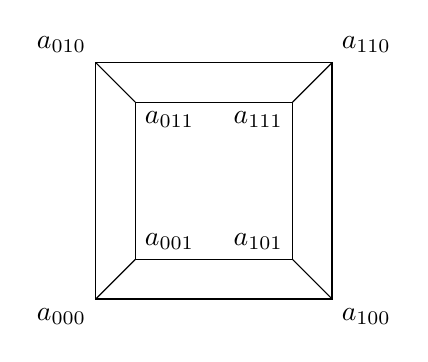
\begin{tikzpicture}
\draw (0,0) -- (3,0) -- (3,3) -- (0,3) -- cycle;
\draw (0.5,0.5) -- (2.5,0.5) -- (2.5,2.5) -- (0.5,2.5) -- cycle;
\draw (0,0) -- (0.5,0.5);
\draw (3,0) -- (2.5,0.5);
\draw (3,3) -- (2.5,2.5);
\draw (0,3) -- (0.5,2.5);
\node[below left] at (0,0) {$a_{000}$};
\node[below right] at (3,0) {$a_{100}$};
\node[above right] at (3,3) {$a_{110}$};
\node[above left] at (0,3) {$a_{010}$};

\node[above right] at (0.5,0.5) {$a_{001}$};
\node[above left] at (2.5,0.5) {$a_{101}$};
\node[below left] at (2.5,2.5) {$a_{111}$};
\node[below right] at (0.5,2.5) {$a_{011}$};
\end{tikzpicture}
\caption{A $2 \times 2 \times 2$-tensor.}
\label{fig:p1p1p1_equations}
\end{figure}

On the other hand, $\dP6$ can be realized as a subvariety of $\P^1 \times \P^1 \times \P^1$ as well. The equations can be described as follows: draw a cube, and let each vertex correspond to a variable. Then the equations of $\P^1 \times \P^1 \times \P^1$ in its Segre embedding are given by taking all ``minors'' along all sides of the cube together with the three long diagonals. See \cref{fig:p1p1p1_equations}. To get $\dP6$, one identifies two opposite corners. Thus in total there are $8-1=7$ variables, just as above. 

The first smoothing is obtained by deforming the equations of $\dP6$ as a subvariety of $\P^2 \times \P^2$.  It can be described by perturbing two of the entries of the matrix below:

\begin{equation}
\label{eq:def2}
\begin{vmatrix}
y & x_1 & x_2 \\
x_4 & y+t_1 & x_3 \\
x_5 & x_6 & y+t_2
\end{vmatrix} \leq 1.
\end{equation}


For $t_1=t_2=0$, we get the cone over $\dP6$, while for generic $t_i$, we get a smooth variety. In fact, we can compute that the discrimant locus (the set of points in $\A^2_{t_1,t_2}$ with singular fiber) are the $t_1$-axis, the $t_2$-axis and the line $t_1=t_2$. Notice that the total space is equal to the cone over $\P^2 \times \P^2$.

Call (any) smooth fiber $X_2$. 

\begin{lemma}
Let $M=\P(\mathcal T_ {\P^2})$ be the projective bundle associated to the tangent sheaf on $\P^2$. Then the smoothing $X_2$ is isomorphic to $M \bs \dP6$. 
\end{lemma}
\begin{proof}
First homogenize the equations \eqref{eq:def2} with respect to $y_1$. Call the homogenized variety $N$. Put $y_0'=y_0$, $y_1' = y_0-ty_1$ and $y_2'=y_0-t_2y_1$. Then we have the relation
\[
h = t_2y_1'-t_1y_2' - (t_1-t_2)y_0' = 0.
\]
Hence we see that $N=\P^2 \times \P^2 \cap (h = 0)$. We can pull back the coordinates $y_i'$ to $\P^2 \times \P^2$. Let $\P^2 \times \P^2$ have coordinates $x_0,x_1,x_2$ and $y_0,y_1,y_2$. Then $h$ pulls back to the equation
\[
(x_0,x_1,x_2) \cdot (-t_1y_2, (t_1-t_2)y_0,t_2y_1) = 0
\]
in $\P^2 \times \P^2$. As long as $t_1 \neq t_2$ and $t_1,t_2 \neq 0$, we can do a change of coordinates in $\P^2_{y_0y_1y_2}$, so that $h$ transforms to
\[
(x_0,x_1,x_2) \cdot(y_0,y_1,y_2) = 0.
\]
Hence we see that $M$ is isomorphic to the total space of the Grassmannian of lines in $\P^2$ (each point in one of the $\P^2$'s give a line in the other $\P^2$). This is in turn isomorphic to $\P(\mathcal T_{\P^2})$, since each tangent vector through a point determines a line through it.

Now, what have we gained by homogenizing? The divisor at infinity is $y_1=0$, which is a $\dP6$ again. In our new coordinates this is equivalent to $y_1'=y_2'=y_0'$. Hence in the coordinates of $\P^2 \times \P^2$, $\dP6$ is given by the two equations $x_1y_0-x_2y_1=x_1y_0-x_0y_2=0$. 
\end{proof}

The other smoothing is the obtained by replacing one of the corners of the cube in \cref{fig:p1p1p1_equations} with $a_{000}'=a_{000}+t$, obtained a one-parameter smoothing. The total space is now that affine cone over $\P^1 \times \P^1 \times \P^1$. 

Call this smoothing $X_1.$

\begin{lemma}
The smoothing $X_1$ is isomorpic to $\P^1 \times \P^1 \times \P^1 \bs \dP6$.
\end{lemma}
\begin{proof}
Homogenize, notice what is gained, then subtract.
\end{proof}

Observe that $\mathcal T(\P^2)$ is homotopy equivalent to $\P^1 \times \P^2$ \todo{source?}. It follows that its Euler characteristic, which is invariant under homotopy, is equal to $2 \times 3=6$.

This information let us calculate the Euler characteristics of the smoothings. Note that $\chi(\P^1)=2$ and $\chi(\mathcal T(\P^2))=6$. By additivity of the Euler characteristics we have $\chi(X_1)=2$ and $\chi(X_2)=0$, since $\chi(\dP6)=6$.

It follows that the two smoothing components correspond to topologically different smoothings. This can explain the obstructedness of the deformations of $X_0$ in \cref{sec:constructions}.


\begin{lemma}
The cohomology ring of $M=\P(\mathcal T_{\P^2})$ is $\Z[x,y]/(x^3,y^2+c_1y+c_2)$, where $x$ and $y$ have degree $2$. In particular, the cohomology of $M$ is given by $(1,0,2,0,2,0,1)$.
\end{lemma}
\begin{proof}
The first claim follows from the Leray-Hirch theorem. See \cite[page 270]{bott_tu}. The next claim follows since $x$ and $y$ both have degree $2$.
\end{proof}

We can use what we know about the topology of these spaces to compute homology groups of the two affine smoothings.

\begin{theorem}
The two affine smoothings are topologically different. The homology groups are:
\begin{center}
\begin{tabular}{ l || c | c | c | c | c | c | c || c }
 Group & 0 & 1 & 2 & 3 & 4 & 5 & 6 & Euler-characteristic \\
\hline
$H^i(X_1,\Z)$ & 1 & 0 & 2 & 1 & 0 & 0 & 0 & 2 \\
$H^i(X_2,\Z)$ & 1 & 0 & 1 & 2 & 0 & 0 & 0  & 0
\end{tabular}
\end{center}
\end{theorem}

\begin{proof}
The singular cohomology of $M=\P^1 \times \P^1 \times \P^1$ is given by $(1,0,3,0,3,0,1)$, which can be computed by the Künneth formula. The cohomology of $\dP6$ is given by $(1,0,4,0,1)$.

We will use the Lefschetz duality theorem \cite{spanier_topology}, which in this case says that $H_q(M \bs dP_6, \Z) \simeq H^{6-q}(M,dP_6,\Z)$. Then the long exact sequence of the pair $(M,dP_6)$ immediately gives $h_0(X_1,\Z)=1$. Similarly, we see that $h_5(X_1,\Z)=h_6(X_1,\Z)=0$, since the map $H^1(M,\Z) \to H^1(D,\Z)$ is an isomorphism.

The other groups depend upon the explicit form of the maps $H^2(M,\Z) \to H^2(D,\Z)$ and $H^4(M,\Z) \to H^4(D,\Z)$.

By Poincaré duality \todo{Find reference}((reference)), the induced map corresponds to intersecting the divisors on $M$ with $dP_6$. Computing, we get that map is given by the following matrix:
\[
H^2(M,\Z) \simeq H_4(M,\Z) \simeq \Z^3 \xrightarrow{
	\begin{pmatrix}
	0 & 1 & 1 \\
	1 & 0 & 1 \\
	1 & 1 & 0 \\
	0 & 0 & 0
	\end{pmatrix}
} \Z^4 \simeq H_2(dP_6,\Z) \simeq H^2(dP_6,\Z).
\]

This is an injective map, and it follows from the long-exact sequence and the Lefschetz theorem that $H_3(X_1) \simeq H^3(M,dP_6) \simeq \Z$, and also that $H_4(X_1)=0$.

Similarly, the map $H^4(M) \to H^4(dP_6)$ is computed to be given by $(a,b,c) \mapsto a+b+c$, since the three $\P^1$'s intersect $\dP6$ in a single point. This map has two-dimensional kernel, and we conclude that $H_2(X_1) \simeq H^4(M,\dP6) = \Z^2$, and that $H^1(X_1)=0$.

The computations for $X_2$ are similar but more involved. We first note that the Picard group of $M=\P(\mathcal T_{\P^2})$ is generated by the pullbacks $F,G$ of the generators of $\Pic(\P^2_{x_0x_1x_2} \times \P^2_{y_0y_1y_2})$. Say $F$ is represented by $V(x_0)$ and $G$ is represented by $V(y_0)$\todo{check transversal intersection with dP6}.

Again we compute the intersections of $F$ and $G$ with $dP_6$. Intersecting with $F$ is computed by decomposing the ideal $(x_0,x_1y_0-x_2y_1,x_1y_0-x_0y_2)$ in $k[x_0,x_1,x_2,y_0,y_1,y_2]$ and saturating by $(x_0,x_1,x_2)$ and $(y_0,y_1,y_2)$. This can either be done by hand or by using \texttt{Macaulay2}. Either way, we find that $\restr{F}{dP_6} = E_3+L_{23} + E_2=H$, using the notation from earlier this chapter. Similarly $\restr{G}{dP_6}=L_{23}+L_{12}+E_2=2H-E_1-E_2-E_3$. Hence the map on cohomology is given by the matrix

\[
H^2(M,\Z) \simeq H_4(M,\Z) \simeq \Z^2 \xrightarrow{
	\begin{pmatrix}
	0 & -1 \\
	0 & -1 \\
	0 & -1  \\
	1 & 2 
	\end{pmatrix}
} \Z^4 \simeq H_2(\dP6,\Z) \simeq H^2(\dP6,\Z).
\]

This is an injective map, and as above, we conclude that $H_3(X_2) \simeq H^3(M,\dP6) \simeq \Z^2$, and also that $H_4(X_1)=0$.


\end{proof}

\begin{remark}
In fact, the Andreotti-Frankel theorem \cite{andreotti_affinecw} states the following: if $V$ is any smooth affine variety of complex dimension $n$, then it has the homotopy type of a CW complex of real dimension $n$. Thus it should be no surprise that $H^j(X_i)=0$ for $j > 3$.
\end{remark}
 

\begin{enumerate}
	\item Talk about 9-16-resolutions
\end{enumerate}

